\documentclass[12pt,a4paper]{ctexart}
\usepackage[margin=2.15cm]{geometry}
\usepackage{amsmath,amssymb,mathtools}
\usepackage{graphicx}
\usepackage{enumitem}
\usepackage{xcolor}
\setlength{\parindent}{2em}
\setlength{\parskip}{0.45em}
\setlist[enumerate]{itemsep=0.35em,topsep=0.35em}
\newcommand{\eps}{\varepsilon}
\newcommand{\dif}{\mathop{}\!\mathrm{d}}
\graphicspath{{figures/}}
\begin{document}

\begin{center}
{\LARGE\heiti 信号与系统大题详细解析}
\end{center}

\section*{1. 时域变换与微分}

\textbf{题目}\quad 已知信号 $f(t+1)$ 的波形如图，试画出
\(\displaystyle \frac{\dif}{\dif t}\left[f\left(\frac{t}{2}-1\right)\right]\) 的波形。

\begin{center}
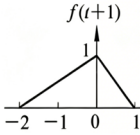
\includegraphics[width=0.34\textwidth]{big_q1_given_signal.png}
\end{center}

\textbf{详细解析}

先把图中已知的信号记为 \(\displaystyle p(t)=f(t+1)\)。由图可直接读出
\[
p(t)=
\begin{cases}
\dfrac{t+2}{2},&-2\leq t<0,\\[0.5em]
1-t,&0\leq t\leq1,\\[0.4em]
0,&\text{其他}.
\end{cases}
\]

由于 \(\displaystyle p(t)=f(t+1)\)，要恢复 $f(t)$，令 $t$ 替换为 $t-1$：
\[
f(t)=p(t-1).
\]
因此，$f(t)$ 的支撑区间由 $[-2,1]$ 向右平移 $1$，变为 $[-1,2]$。代入可得
\[
f(t)=
\begin{cases}
\dfrac{t+1}{2},&-1\leq t<1,\\[0.55em]
2-t,&1\leq t\leq2,\\[0.4em]
0,&\text{其他}.
\end{cases}
\]

现在令
\[
g(t)=f\left(\frac{t}{2}-1\right).
\]
设 \(\displaystyle \tau=\frac{t}{2}-1\)。把 $f(\tau)$ 的关键时刻 \(\tau=-1,1,2\) 映射到 $t$ 轴：
\[
\tau=-1\Rightarrow t=0,\qquad
\tau=1\Rightarrow t=4,\qquad
\tau=2\Rightarrow t=6.
\]

于是：
\[
g(t)=
\begin{cases}
\dfrac{t}{4},&0\leq t<4,\\[0.6em]
3-\dfrac{t}{2},&4\leq t\leq6,\\[0.6em]
0,&\text{其他}.
\end{cases}
\]

最后逐段求导：
\[
\boxed{
\frac{\dif}{\dif t}\left[f\left(\frac{t}{2}-1\right)\right]
=
\begin{cases}
\dfrac14,&0<t<4,\\[0.55em]
-\dfrac12,&4<t<6,\\[0.55em]
0,&\text{其他}.
\end{cases}}
\]

这里 $g(t)$ 在 $t=0,4,6$ 均连续，只是斜率发生突变，所以导数中\textbf{没有}冲激项。作图时，在 $0<t<4$ 画高度为 $1/4$ 的水平线，在 $4<t<6$ 画高度为 $-1/2$ 的水平线，其余时间为 $0$。

\newpage
\section*{2. 并联--串联系统的总冲激响应}

\textbf{题目}\quad 已知
\(\displaystyle h_1(t)=\eps(t)\)、
\(\displaystyle h_2(t)=\delta(t-1)\)、
\(\displaystyle h_3(t)=-\delta(t)\)，系统结构如图，求总系统冲激响应 $h(t)$。

\begin{center}
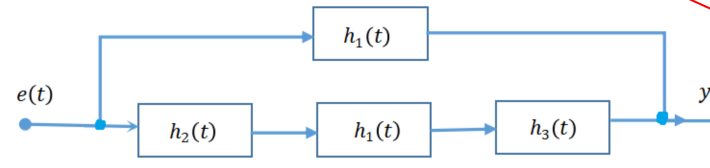
\includegraphics[width=0.88\textwidth]{big_q2_system_block.png}
\end{center}

\textbf{详细解析}

总系统由上、下两条并联支路构成，因此总冲激响应等于两条支路冲激响应之和：
\[
h(t)=h_{\text{上}}(t)+h_{\text{下}}(t).
\]

输入取单位冲激 \(\displaystyle e(t)=\delta(t)\)。常用卷积性质为：
\[
\delta(t)*x(t)=x(t),
\qquad
x(t)*\delta(t-t_0)=x(t-t_0),
\qquad
x(t)*[-\delta(t)]=-x(t).
\]

\textbf{上支路：}

上支路只有 $h_1(t)$，所以
\[
h_{\text{上}}(t)=\delta(t)*h_1(t)
=\delta(t)*\eps(t)
=\eps(t).
\]

\textbf{下支路：}

下支路依次串联 $h_2(t)$、$h_1(t)$、$h_3(t)$。为了看清每一步，设各级输出分别为 $x_1(t)$、$x_2(t)$、$x_3(t)$。

首先经过单位延时器：
\[
x_1(t)=\delta(t)*\delta(t-1)=\delta(t-1).
\]
这一步只是把输入冲激延时到 $t=1$。

接着经过积分器：
\[
x_2(t)=x_1(t)*\eps(t)
=\delta(t-1)*\eps(t)
=\eps(t-1).
\]
所以进入 $h_3(t)$ 的信号已经是延时阶跃 \(\eps(t-1)\)，而不是冲激。这里并不矛盾：$h_3(t)=-\delta(t)$ 是第三个子系统的\textbf{冲激响应}，它可以作用于任何输入信号。

最后经过倒相器：
\[
x_3(t)=\eps(t-1)*[-\delta(t)]
=-\eps(t-1).
\]
因此，下支路输出为
\[
h_{\text{下}}(t)=-\eps(t-1).
\]

两条并联支路相加：
\[
\boxed{
h(t)=\eps(t)-\eps(t-1).}
\]

该结果表示：系统在 $0\leq t<1$ 的冲激响应为 $1$，其他时刻为 $0$。

\newpage
\section*{3. 利用积分性质求梯形信号频谱}

\textbf{题目}\quad 利用傅里叶变换的积分性质，求下列梯形信号 $f(t)$ 的频谱 $F(\omega)$。

\begin{center}
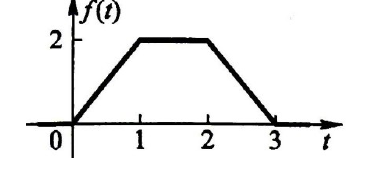
\includegraphics[width=0.40\textwidth]{big_q3_trapezoid.png}
\end{center}

\textbf{详细解析}

\textbf{思路：}梯形信号分段较多，但求导后会变成两个矩形脉冲。先对 $f(t)$ 求导得到 $f'(t)$，求出 $f'(t)$ 的频谱，再利用\textbf{时域积分性质}由 $\mathcal F\{f'(t)\}$ 还原 $F(\omega)$。

从图中可读出：

\begin{itemize}
\item 在 $0<t<1$，信号从 $0$ 线性上升到 $2$，斜率为 $2$；
\item 在 $1<t<2$，信号保持常数 $2$，斜率为 $0$；
\item 在 $2<t<3$，信号从 $2$ 线性下降到 $0$，斜率为 $-2$；
\item 其他时间信号为 $0$。
\end{itemize}

因此
\[
f'(t)=
\begin{cases}
2,&0<t<1,\\
0,&1<t<2,\\
-2,&2<t<3,\\
0,&\text{其他}.
\end{cases}
\]

用阶跃函数表示为
\[
f'(t)=2[\eps(t)-\eps(t-1)]-2[\eps(t-2)-\eps(t-3)].
\]

先求 $f'(t)$ 的频谱：
\begin{align*}
\mathcal F\{f'(t)\}
&=2\int_0^1e^{-j\omega t}\dif t-2\int_2^3e^{-j\omega t}\dif t\\
&=\frac{2}{j\omega}
\left(1-e^{-j\omega}-e^{-j2\omega}+e^{-j3\omega}\right).
\end{align*}

由于 $f(t)=\displaystyle\int_{-\infty}^{t}f'(\tau)\dif\tau$，由\textbf{时域积分性质}
\[
\mathcal F\left\{\int_{-\infty}^{t}g(\tau)\dif\tau\right\}
=\frac{G(\omega)}{j\omega}+\pi G(0)\delta(\omega),
\]
取 $g(t)=f'(t)$。注意 $f'(t)$ 的直流分量
\[
\mathcal F\{f'(t)\}\big|_{\omega=0}
=\int_{-\infty}^{\infty}f'(t)\dif t=0
\]
（正负面积抵消），故 $\pi G(0)\delta(\omega)$ 项为零，得
\[
\boxed{
F(\omega)=\frac{\mathcal F\{f'(t)\}}{j\omega}
=\frac{2}{(j\omega)^2}
\left(1-e^{-j\omega}-e^{-j2\omega}+e^{-j3\omega}\right).}
\]

还可以把括号内因式分解：
\[
1-e^{-j\omega}-e^{-j2\omega}+e^{-j3\omega}
=\left(1-e^{-j\omega}\right)\left(1-e^{-j2\omega}\right).
\]
进而得到等价形式：
\[
\boxed{
F(\omega)=
\frac{8e^{-j\frac{3\omega}{2}}
\sin\frac{\omega}{2}\sin\omega}{\omega^2}.}
\]

在 $\omega=0$ 处，频谱值等于时域面积。梯形面积为
\[
\frac12\times1\times2+1\times2+\frac12\times1\times2=4,
\]
所以 \(\displaystyle F(0)=4\)。

\newpage
\section*{4. 串联 RLC 电路的零状态响应}

\textbf{题目}\quad 如图串联 RLC 电路中，
$R=5\,\Omega$，$L=1\,\mathrm H$，$C=\frac16\,\mathrm F$。
零初始条件下输入 \(\displaystyle f(t)=12\eps(t)\,\mathrm V\)，求电容电压 $u_C(t)$。

\begin{center}
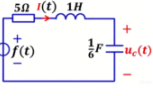
\includegraphics[width=0.28\textwidth]{big_q4_rlc_circuit.png}
\end{center}

\textbf{详细解析}

由于电路为零初始状态，可以直接使用 $s$ 域阻抗模型：
\[
Z_R=R=5,
\qquad
Z_L=sL=s,
\qquad
Z_C=\frac{1}{sC}=\frac{6}{s}.
\]

输入电压的拉普拉斯变换为
\[
F(s)=\mathcal L\{12\eps(t)\}=\frac{12}{s}.
\]

串联总阻抗为
\begin{align*}
Z_{\text{总}}(s)
&=Z_R+Z_L+Z_C\\
&=5+s+\frac6s\\
&=\frac{s^2+5s+6}{s}\\
&=\frac{(s+2)(s+3)}{s}.
\end{align*}

因此串联支路电流为
\begin{align*}
I(s)
&=\frac{F(s)}{Z_{\text{总}}(s)}\\
&=\frac{12/s}{(s^2+5s+6)/s}\\
&=\frac{12}{(s+2)(s+3)}.
\end{align*}

电容电压等于电流乘以电容阻抗：
\begin{align*}
U_C(s)
&=I(s)Z_C\\
&=\frac{12}{(s+2)(s+3)}\cdot\frac6s\\
&=\frac{72}{s(s+2)(s+3)}.
\end{align*}

进行部分分式展开：
\[
\frac{72}{s(s+2)(s+3)}
=\frac{A}{s}+\frac{B}{s+2}+\frac{C}{s+3}.
\]

代入 $s=0$：
\[
72=A\cdot2\cdot3\quad\Rightarrow\quad A=12.
\]
代入 $s=-2$：
\[
72=B(-2)(1)\quad\Rightarrow\quad B=-36.
\]
代入 $s=-3$：
\[
72=C(-3)(-1)\quad\Rightarrow\quad C=24.
\]

故
\[
U_C(s)=\frac{12}{s}-\frac{36}{s+2}+\frac{24}{s+3}.
\]

利用 \(\displaystyle \mathcal L^{-1}\{1/s\}=\eps(t)\) 和
\(\displaystyle \mathcal L^{-1}\{1/(s+a)\}=e^{-at}\eps(t)\)，得到
\[
\boxed{
u_C(t)=\left(12-36e^{-2t}+24e^{-3t}\right)\eps(t)\ \mathrm V.}
\]

检验：
\[
u_C(0^+)=12-36+24=0,
\]
符合零初始条件下电容电压不能突变的物理规律；当 $t\to\infty$ 时，
\[
u_C(\infty)=12\,\mathrm V,
\]
符合直流稳态下电容开路、其两端电压等于输入直流电压的结论。

\newpage
\section*{5. 由系统函数求微分方程、零输入响应和全响应}

\textbf{题目}\quad 已知
\[f(t)=e^{-t}\eps(t),\qquad y(0^-)=1,\qquad y'(0^-)=2,\]
以及
\[
H(s)=\frac{3s+1}{s^2+5s+6}.
\]
求对应微分方程、零输入响应、零状态响应和全响应。

\textbf{详细解析}

\textbf{第一步：由 $H(s)$ 写微分方程。}

零初始条件下，系统函数满足
\[
H(s)=\frac{Y_{\mathrm{zs}}(s)}{F(s)}
=\frac{3s+1}{s^2+5s+6}.
\]
因此
\[
(s^2+5s+6)Y(s)=(3s+1)F(s).
\]
将 $sY(s)$、$s^2Y(s)$ 分别对应到 $y'(t)$、$y''(t)$，将 $sF(s)$ 对应到 $f'(t)$，得到
\[
\boxed{y''(t)+5y'(t)+6y(t)=3f'(t)+f(t).}
\]

\textbf{第二步：求零输入响应。}

零输入响应时令 $f(t)=0$。对微分方程作拉普拉斯变换，并带入初始条件：
\begin{align*}
&\left[s^2Y(s)-sy(0^-)-y'(0^-)\right]
+5\left[sY(s)-y(0^-)\right]+6Y(s)=0\\
\Rightarrow\quad
&(s^2+5s+6)Y_{\mathrm{zi}}(s)=s+7.
\end{align*}

所以
\[
Y_{\mathrm{zi}}(s)=\frac{s+7}{(s+2)(s+3)}.
\]
部分分式展开：
\[
\frac{s+7}{(s+2)(s+3)}
=\frac5{s+2}-\frac4{s+3}.
\]
反变换得到
\[
\boxed{
y_{\mathrm{zi}}(t)=\left(5e^{-2t}-4e^{-3t}\right)\eps(t).}
\]

\textbf{第三步：求零状态响应。}

零状态响应时初始条件取零，直接使用
\[
Y_{\mathrm{zs}}(s)=H(s)F(s).
\]
因为
\[
F(s)=\mathcal L\{e^{-t}\eps(t)\}=\frac{1}{s+1},
\]
所以
\[
Y_{\mathrm{zs}}(s)
=\frac{3s+1}{(s+1)(s+2)(s+3)}.
\]
进行部分分式展开：
\[
\frac{3s+1}{(s+1)(s+2)(s+3)}
=-\frac1{s+1}+\frac5{s+2}-\frac4{s+3}.
\]
因此
\[
\boxed{
y_{\mathrm{zs}}(t)=
\left(-e^{-t}+5e^{-2t}-4e^{-3t}\right)\eps(t).}
\]

\textbf{第四步：叠加得到全响应。}

线性系统的全响应为
\[
y(t)=y_{\mathrm{zi}}(t)+y_{\mathrm{zs}}(t).
\]
故
\[
\boxed{
y(t)=
\left(-e^{-t}+10e^{-2t}-8e^{-3t}\right)\eps(t).}
\]

\newpage
\section*{6. 离散时间卷积和与移位}

\textbf{题目}\quad 已知
\[
f_1(k)=2^{-(k+1)}\eps(k+1),
\qquad
f_2(k)=\eps(k-2),
\]
求 \(\displaystyle f_1(k)*f_2(k)\)。

\textbf{详细解析}

先把两个序列写成“未移位基本序列”的形式。令
\[
x(k)=2^{-k}\eps(k),
\qquad
u(k)=\eps(k).
\]
则
\[
f_1(k)=x(k+1),
\qquad
f_2(k)=\nu(k-2).
\]

先求未移位卷积
\[
y_1(k)=x(k)*\nu(k).
\]
由卷积和定义：
\begin{align*}
y_1(k)
&=\sum_{i=-\infty}^{\infty}x(i)\nu(k-i)\\
&=\sum_{i=-\infty}^{\infty}2^{-i}\eps(i)\eps(k-i).
\end{align*}

条件 \(\eps(i)=1\) 要求 $i\geq0$；条件 \(\eps(k-i)=1\) 要求 $i\leq k$。因此，当 $k\geq0$ 时，求和范围为 $0\leq i\leq k$：
\begin{align*}
y_1(k)
&=\sum_{i=0}^{k}2^{-i}\\
&=1+\frac12+\frac14+\cdots+2^{-k}\\
&=\frac{1-(1/2)^{k+1}}{1-1/2}\\
&=2-2^{-k}.
\end{align*}

所以
\[
y_1(k)=\left(2-2^{-k}\right)\eps(k).
\]

接下来处理移位。$f_1(k)=x(k+1)$ 相对于 $x(k)$ 向左移动 $1$；$f_2(k)=\nu(k-2)$ 相对于 $\nu(k)$ 向右移动 $2$。卷积后总移位量为
\[
(-1)+2=1.
\]
即结果相对于 $y_1(k)$ 向右移动 $1$，所以
\[
f_1(k)*f_2(k)=y_1(k-1).
\]

代入 $y_1(k)$：
\[
\boxed{
f_1(k)*f_2(k)
=\left[2-2^{-(k-1)}\right]\eps(k-1).}
\]

\newpage
\section*{7. 给定不同 ROC 的 $Z$ 反变换}

\textbf{题目}\quad 已知
\[
F(z)=\frac{3z^2}{(z+1)(z-2)},
\]
分别求在 \(\displaystyle |z|>2\)、\(\displaystyle |z|<1\)、\(\displaystyle 1<|z|<2\) 时对应的反变换 $f(k)$。

\textbf{详细解析}

同一个代数式 $F(z)$，如果收敛域 ROC 不同，反变换可能不同。因此必须先做部分分式展开，再根据 ROC 分别判断每一项是右边序列还是左边序列。

先展开：
\[
F(z)=\frac{z}{z+1}+2\frac{z}{z-2}.
\]

使用基本变换对：
\[
\frac{z}{z-a}
\longleftrightarrow
\begin{cases}
a^k\eps(k),&|z|>|a|,\\[0.45em]
-a^k\eps(-k-1),&|z|<|a|.
\end{cases}
\]

这里两个极点分别为
\[
z=-1,\qquad z=2.
\]

\textbf{(1) ROC：$|z|>2$}

该 ROC 位于两个极点之外，因此两项都取右边序列：
\[
\frac{z}{z+1}
\longleftrightarrow
(-1)^k\eps(k),
\]
\[
2\frac{z}{z-2}
\longleftrightarrow
2\cdot2^k\eps(k)=2^{k+1}\eps(k).
\]
故
\[
\boxed{
f(k)=\left[(-1)^k+2^{k+1}\right]\eps(k),
\qquad |z|>2.}
\]

\textbf{(2) ROC：$|z|<1$}

该 ROC 位于两个极点之内，因此两项都取左边序列：
\[
\frac{z}{z+1}
\longleftrightarrow
-(-1)^k\eps(-k-1),
\]
\[
2\frac{z}{z-2}
\longleftrightarrow
-2\cdot2^k\eps(-k-1)=-2^{k+1}\eps(-k-1).
\]
故
\[
\boxed{
f(k)=-\left[(-1)^k+2^{k+1}\right]\eps(-k-1),
\qquad |z|<1.}
\]

\textbf{(3) ROC：$1<|z|<2$}

对于极点 $z=-1$，ROC 在其外侧，因此对应右边序列；对于极点 $z=2$，ROC 在其内侧，因此对应左边序列：
\[
\frac{z}{z+1}
\longleftrightarrow
(-1)^k\eps(k),
\]
\[
2\frac{z}{z-2}
\longleftrightarrow
-2^{k+1}\eps(-k-1).
\]
所以
\[
\boxed{
f(k)=(-1)^k\eps(k)-2^{k+1}\eps(-k-1),
\qquad 1<|z|<2.}
\]

\end{document}
